
\section{紧空间上的类梯度流}
\label{sec:gradient-flows}

\hzsync{theorem}{6}%
\hzsync{proposition}{8}%
\hzsync{definition}{2}%
\hzsync{equation}{47}%

下文中，$X$ 是一个\trCompact{}\trMetric{}空间。$X$ 上的一个\trFlow{}是一个%
连续映射 $\varphi:\R\times X\to X$，$(t,x)\mapsto\varphi(t,x)=\varphi^{t}(x)$，%
它满足
\begin{equation}\label{eq:flow-semigroup}
\begin{aligned}
\varphi^{t}\Bigl(\varphi^{s}(x)\Bigr)\ &=\ \varphi^{t+s}(x)\\
\varphi^{0}(x)\ &=\ x
\end{aligned}
\end{equation}
对一切 $t,s\in\R$ 与 $x\in X$。一个例子是\trCompact{}\trManifold{}上一个可微%
\trVectorField{}的\trFlow。我们将使用记号
\[
\varphi^{t}(x)\ =\ x\cdot t
\]
并且，对子集 $M\subset X$ 与 $B\subset\R$，缩记%
$M\cdot B:=\bigl\{\,x\cdot t\ \bigm|\ x\in M\ \text{且}\ t\in B\,\bigr\}$。若%
$x\in X$，则从 $\R$ 到 $X$ 的映射
\[
t\ \mapsto\ \varphi^{t}(x)\ =\ x\cdot t
\]
称为通过点 $x\in X$ 的解。通过 $x$ 的正（相应地，负）解的像将记作%
$\gamma^{\pm}(x)=x\cdot\R^{\pm}$，并且我们令 $\gamma(x)=x\cdot\R$。由%
\eqref{eq:flow-semigroup}，每个点 $x\in X$ 都恰属于一条\trOrbit{} $\gamma(x)$。%
由
\[
x\cdot t\ =\ x\,,\qquad t\in\R
\]
所刻画的那些特定的常值解，称为该\trFlow{}的\trRestPoint{}或\trFixedPoint；%
显然此时 $\gamma(x)=\{x\}$。为了描述一个\trFlow{}的整体\trOrbit{}结构，回顾%
通过 $x\in X$ 的解的\textbf{正\trLimitSet}（positive limit set）$\omega(x)$ 与%
\textbf{负\trLimitSet}（negative limit set）$\omega^{*}(x)$ 的概念是有用的。

\begin{definition}\label{def:limit-sets}
\begin{align*}
\omega(x)\ &=\ \bigl\{\,y\in X\ \bigm|\ \exists\ t_{j}\to+\infty\ \text{使得}\ x\cdot t_{j}\to y\,\bigr\}\\
\omega^{*}(x)\ &=\ \bigl\{\,y\in X\ \bigm|\ \exists\ t_{j}\to-\infty\ \text{使得}\ x\cdot t_{j}\to y\,\bigr\}.
\end{align*}
\end{definition}

我们来总结这些\trLimitSet{}的众所周知性质。回忆 $X$ 是\trCompact{}的。

\begin{proposition}\label{prop:limit-sets}
若 $x\in X$，则\trLimitSet $\omega(x)$ 与 $\omega^{*}(x)$ 非空、\trCompact、%
\trConnected{}且在该\trFlow{}下\trInvariant，即 $\omega(x)\cdot t=\omega(x)$%
对一切 $t\in\R$ 成立。此外，
\begin{equation}\label{eq:limit-convergence}
\begin{aligned}
x\cdot t\ \ \longrightarrow\ \ \omega(x)\qquad&\text{当 }t\to+\infty\\
x\cdot t\ \ \longrightarrow\ \ \omega^{*}(x)\qquad&\text{当 }t\to-\infty\,.
\end{aligned}
\end{equation}
\end{proposition}

\begin{proof}
若 $t_{j}\to\infty$，则序列 $x\cdot t_{j}$ 有一个收敛的子序列，于是%
$\omega(x)\neq\emptyset$。假设 \eqref{eq:limit-convergence} 不成立；那么存在一个%
开\trNeighborhood{} $U\supset\omega(x)$ 与一个序列 $t_{j}\to\infty$ 使得%
$x\cdot t_{j}\in X\setminus U$。于是对某个子序列 $x\cdot t_{j}\to y\in X\setminus U$。%
按定义 $y\in\omega(x)$，这与 $\omega(x)\subset U$ 相矛盾。若 $\omega(x)$ 不%
\trConnected，则 $\omega(x)=\omega_{1}\cup\omega_{2}$，其中 $\omega_{j}\subset X$%
是两个非空、\trCompact{}且相互\trDisjoint{}的子集。取诸 $\omega_{j}$（$j=1,2$）%
相互\trDisjoint{}的开\trNeighborhood{} $U_{j}$；于是由%
\eqref{eq:limit-convergence}，$x\cdot t\to\omega(x)$，从而对 $t\geq t^{*}$ 我们有%
$x\cdot t\in U_{1}\cup U_{2}$，并且 $\gamma^{+}(x\cdot t)\cap U_{j}\neq\emptyset$%
（$j=1,2$）。结果，集合 $\gamma^{+}(x\cdot t)$ 不\trConnected，这与「$\R$ 中%
一个区间的连续像是\trConnected{}的」这一事实相矛盾。诸\trLimitSet{}的\trInvariance{}%
则是该\trFlow{}之\trContinuity{}的一个直接推论。
\end{proof}

现在我们进一步假设该\trFlow{}是\trGradientLike{}的，即我们要求存在一个连续%
函数 $V:X\to\R$，它沿每条非常值解都严格\trMonotone{}递减：
\[
t>s\ \Longrightarrow\ V(x\cdot t)<V(x\cdot s)\,.
\]
这样的函数通常称为该\trFlow{}的一个\trLyapunov{}函数。一个众所周知的特殊%
例子，是\trCompact{}\trRiemann\trManifold{}上由\trSmooth{}\trGradient{}向量场%
$\dot{x}=-\nabla V(x)$ 生成的\trFlow。

\begin{proposition}\label{prop:limit-rest-points}
若该\trFlow{}是\trGradientLike{}的，则每条解的\trLimitSet{}都由\trRestPoint{}组成：
\[
\omega(x)\ \text{与}\ \omega^{*}(x)\ \subset\ \{\,\text{驻点}\,\}\,,
\]
对每个 $x\in X$。
\end{proposition}

\begin{proof}
由于 $V(x\cdot t)$ \trMonotone{}递减，极限
\[
\lim_{t\to+\infty}\ V(x\cdot t)\ =\ \inf\,\bigl\{\,V(x\cdot t)\ \bigm|\ t\geq0\,\bigr\}\ =:\ d
\]
在 $\R$ 中存在。若 $y\in\omega(x)$，则由 $V$ 的\trContinuity{}我们得出%
$V(y)=d$，从而鉴于 $\omega(x)$ 在该\trFlow{}下的\trInvariance，$V(y\cdot t)=d$%
对每个 $t\in\R$ 成立。由假设，$V$ 沿非常值解严格递减，故 $y$ 必如所断言是一个%
\trRestPoint。
\end{proof}

若该\trGradientLike\trFlow{}只拥有孤立的\trRestPoint，则它们只有有限多个，%
设为 $\{x_{1},\ldots,x_{N}\}$，并且由该命题我们得出：每条非常值解都连接两个%
互不相同的\trRestPoint。每个点 $x\in X$ 在该\trFlow{}下于正向与反向时间上都%
趋于一个特定的\trRestPoint。

该\trFlow{}的诸\trRestPoint{}与 $X$ 的\trTopology{}性质紧密相关，这并不令人%
惊讶。的确，我们将从\cref{prop:limit-rest-points}引出下述存在性命题，它已在%
6.2 节中作为\cref{thm:rest-point-estimate}表述过。

\begin{theorem}[\trLjusternik-\trSchnirelman]\label{thm:gradient-rest-points}
对\trCompact{}\trMetric{}空间上的每个\trGradientLike\trFlow，我们都有
\[
\#\ \{\ \text{驻点}\ \}\ \geq\ \text{\trCupLength}\,(X)\ +\ 1\,.
\]
\end{theorem}

\noindent\begin{minipage}{\linewidth}
\centering
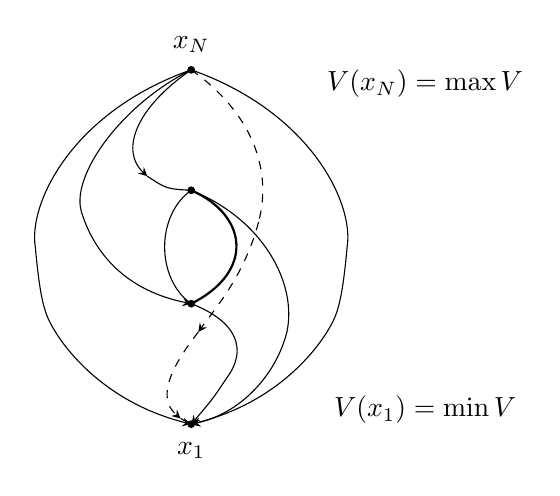
\begin{tikzpicture}[>=stealth,scale=0.9]
  \draw (0,2.5) .. controls (-1.7,1.9) and (-2.3,0.6) .. (-2.2,0);
  \draw (-2.2,0) .. controls (-2.15,-0.55) and (-2.1,-0.85) .. (-2.0,-1.05);
  \draw[->] (-2.0,-1.05) .. controls (-1.8,-1.45) and (-1.2,-2.2) .. (0,-2.5);
  \draw (0,2.5) .. controls (1.7,1.9) and (2.3,0.6) .. (2.2,0);
  \draw (2.2,0) .. controls (2.15,-0.55) and (2.1,-0.85) .. (2.0,-1.05);
  \draw[->] (2.0,-1.05) .. controls (1.8,-1.45) and (1.2,-2.2) .. (0,-2.5);
  \draw[->] (0,2.5) .. controls (-0.8,1.95) and (-1.0,1.35) .. (-0.62,1.0);
  \draw (-0.62,1.0) .. controls (-0.35,0.82) .. (0,0.8);
  \draw[dashed] (0,2.5) .. controls (0.85,1.9) and (1.15,1.1) .. (0.95,0.35);
  \draw[dashed,->] (0.95,0.35) .. controls (0.75,-0.4) and (0.35,-0.85) .. (0.1,-1.2);
  \draw[dashed,->] (0.1,-1.2) .. controls (-0.45,-1.9) and (-0.4,-2.2) .. (-0.15,-2.42);
  \draw[dashed] (-0.15,-2.42) -- (0,-2.5);
  \draw[thin] (0,0.8) .. controls (-0.5,0.45) and (-0.5,-0.45) .. (0,-0.8);
  \draw[thick] (0,0.8) .. controls (0.8,0.45) and (0.9,-0.35) .. (0,-0.8);
  \draw (0,2.5) .. controls (-1.0,2.0) and (-1.7,1.0) .. (-1.55,0.5);
  \draw[->] (-1.55,0.5) .. controls (-1.4,0.0) and (-1.0,-0.6) .. (0,-0.8);
  \draw (0,0.8) .. controls (1.0,0.4) and (1.5,-0.5) .. (1.35,-1.2);
  \draw[->] (1.35,-1.2) .. controls (1.2,-1.8) and (0.7,-2.35) .. (0,-2.5);
  \draw (0,-0.8) .. controls (0.65,-1.05) and (0.8,-1.45) .. (0.5,-1.85);
  \draw[->] (0.5,-1.85) .. controls (0.3,-2.15) .. (0,-2.5);
  \fill (0,2.5) circle (0.055);
  \fill (0,0.8) circle (0.055);
  \fill (0,-0.8) circle (0.055);
  \fill (0,-2.5) circle (0.055);
  \node[above] at (0,2.6) {$x_{N}$};
  \node[below] at (0,-2.62) {$x_{1}$};
  \node at (3.3,2.3) {$V(x_{N})=\max V$};
  \node at (3.3,-2.3) {$V(x_{1})=\min V$};
\end{tikzpicture}

图 6.7a
\end{minipage}

\cref{thm:gradient-rest-points}将立刻由关于诸\trFlow{}之%
\textbf{\trMorse{}分解}（Morse decomposition）的一个一般的定性命题推出，%
此处这些\trFlow{}不必是\trGradientLike{}的。该命题取自 [55]。

\begin{definition}\label{def:morse-decomposition}
一个\trFlow{}的\trMorse{}分解是互\trDisjoint、\trCompact{}且\trInvariant{}的%
子集 $M_{j}\subset X$ 所成的一个有限族 $\{M_{j}\}_{j\in I}$，这些子集可以排序，%
比如说排成 $(M_{1},M_{2},\ldots,M_{k})$，使得下述性质成立：对每个
\[
x\in X\setminus\bigcup_{j\in I}M_{j}
\]
存在一对指标 $i<j$，使得 $\omega(x)\subset M_{i}$ 且 $\omega^{*}(x)\subset M_{j}$。
\end{definition}

\begin{theorem}\label{thm:morse-decomposition-inequality}
设 $\{M_{j}\}_{j\in I}$ 是\trCompact{}空间 $X$ 上一个\trFlow{}的\trMorse{}分解。%
那么
\begin{equation}\label{eq:morse-inequality}
CL(X)\ +\ 1\ \leq\ \sum_{j\in I}\bigl\{\,CL(M_{j})+1\,\bigr\}\,.
\end{equation}
\end{theorem}

特别地，若 $|I|<CL(X)+1$，则某个\trCompact{}\trInvariant{}集 $M_{j}$ 便具有%
非平凡的\trAlexander-\trSpanier{}上同调，从而其点的基数至少为%
\textbf{\trContinuum}（continuum）。

我们已把一个空间 $S$ 的\trCupLength{}缩记为 $CL(S)$。此处不要求该\trFlow{}是%
\trGradientLike{}的。我们把此定理的证明搁置一下，先证明%
\cref{thm:gradient-rest-points}。

\begin{proof}[\cref*{thm:gradient-rest-points}的证明]
以 $V$ 表示该\trGradientLike\trFlow{}的\trLyapunov{}函数，并设它只有有限多个%
\trRestPoint。于是诸\trRestPoint{}可以排序，使得%
$V(x_{1})\leq V(x_{2})\leq\cdots\leq V(x_{k})$。由于 $V$ 沿诸非常值解严格递减，%
诸\trRestPoint{} $\{x_{1},\ldots,x_{k}\}$ 按\cref{prop:limit-rest-points}构成该%
\trFlow{}的一个\trMorse{}分解。由于 $CL(\{x_{j}\})=0$，我们从%
\cref{thm:morse-decomposition-inequality}得出
\[
CL(X)\ +\ 1\ \leq\ \sum_{1\leq j\leq k}1
\]
从而\trRestPoint{}的个数确实必须大于或等于 $CL(X)+1$，于是%
\cref{thm:gradient-rest-points}得证。
\end{proof}

\begin{proof}[\cref*{thm:morse-decomposition-inequality}的证明]
首先观察到：$X$ 的任何\trMorse{}分解都可以这样得到——先把 $X$ 分解为两个%
集合，再分解其中的一个，如此继续，直至达到所需的分解。的确，设%
$\{M_{1},M_{2},\ldots,M_{k}\}$ 是 $X$ 的一个有序\trMorse{}分解。那么定义子集
\[
X_{1}=\bigl\{\,x\in X\ \bigm|\ \omega(x)\cup\omega^{*}(x)\subset%
M_{1}\cup M_{2}\cup\cdots\cup M_{k-1}\,\bigr\}.
\]
这个集合是\trCompact{}的且在该\trFlow{}下\trInvariant，从而 $\{X_{1},M_{k}\}$%
构成 $X$ 的一个分成两个集合的有序\trMorse{}分解。因此，只须对该定理就分解成%
两个集合的情形给出证明。于是设 $\{M_{1},M_{2}\}$ 是 $X$ 的一个有序%
\trMorse{}分解。从这个定义我们得出：存在 $M_{1}$ 的一个\trCompact%
\trNeighborhood{} $S_{1}$ 与 $M_{2}$ 在 $X$ 中的一个\trCompact\trNeighborhood{}%
$S_{2}$，满足 $S_{1}\cup S_{2}=X$，而且更有
\[
M_{1}\ =\ \bigcap_{t>0}S_{1}\cdot t\qquad\text{而}\qquad M_{2}\ =\ %
\bigcap_{t>0}S_{2}\cdot(-t)\,.
\]
从而，注意到对每个 $t\in\R$ 都有 $\check{H}^{*}(S_{1}\cdot t)=\check{H}^{*}(S_{1})$%
（$S_{2}$ 类似），我们借\trAlexander-\trSpanier{}上同调的\trContinuity%
得出 $\check{H}^{*}(S_{1})=\check{H}^{*}(M_{1})$ 与%
$\check{H}^{*}(S_{2})=\check{H}^{*}(M_{2})$。因此，采用缩记%
$c(S)=CL(S)+1$，只须对 $S_{1}\cup S_{2}=X$ 证明%
$c(S_{1})+c(S_{2})\geq c(X)$。这将由下述拓扑学的观察得出：

\begin{lemma}\label{lem:cup-product-kernel}
设 $S_{1}$、$S_{2}$ 与 $S$ 为三个\trCompact{}集，且 $S_{1}\cup S_{2}\subset S$。%
以 $i_{1}:S_{1}\to S$、%
$i_{2}:S_{2}\to S$ 与 $i:S_{1}\cup S_{2}\to S$ 表示诸\trInclusionMapping。设%
$\alpha,\beta\in\check{H}^{*}(S)$。那么 $i_{1}^{*}(\alpha)=0$ 与%
$i_{2}^{*}(\beta)=0$ 蕴含 $i^{*}(\alpha\cup\beta)=0$。
\end{lemma}

\begin{proof}[\cref*{lem:cup-product-kernel}的证明]
考虑下图：
\begin{center}
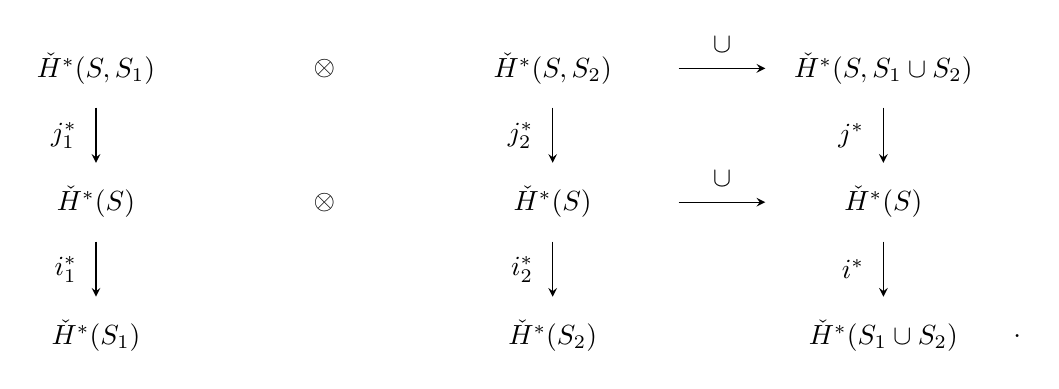
\begin{tikzpicture}[>=stealth]
  \node (a) at (0,0) {$\check{H}^{*}(S,S_{1})$};
  \node at (2.9,0) {$\otimes$};
  \node (b) at (5.8,0) {$\check{H}^{*}(S,S_{2})$};
  \node (c) at (10.0,0) {$\check{H}^{*}(S,S_{1}\cup S_{2})$};
  \node (d) at (0,-1.7) {$\check{H}^{*}(S)$};
  \node at (2.9,-1.7) {$\otimes$};
  \node (e) at (5.8,-1.7) {$\check{H}^{*}(S)$};
  \node (f) at (10.0,-1.7) {$\check{H}^{*}(S)$};
  \node (g) at (0,-3.4) {$\check{H}^{*}(S_{1})$};
  \node (h) at (5.8,-3.4) {$\check{H}^{*}(S_{2})$};
  \node (i) at (10.0,-3.4) {$\check{H}^{*}(S_{1}\cup S_{2})$};
  \draw[->] (7.4,0) -- (8.5,0);
  \node[above] at (7.95,0.08) {$\cup$};
  \draw[->] (7.4,-1.7) -- (8.5,-1.7);
  \node[above] at (7.95,-1.62) {$\cup$};
  \draw[->] (0,-0.5) -- (0,-1.2);
  \node[left] at (-0.12,-0.85) {$j_{1}^{*}$};
  \draw[->] (5.8,-0.5) -- (5.8,-1.2);
  \node[left] at (5.68,-0.85) {$j_{2}^{*}$};
  \draw[->] (10.0,-0.5) -- (10.0,-1.2);
  \node[left] at (9.88,-0.85) {$j^{*}$};
  \draw[->] (0,-2.2) -- (0,-2.9);
  \node[left] at (-0.12,-2.55) {$i_{1}^{*}$};
  \draw[->] (5.8,-2.2) -- (5.8,-2.9);
  \node[left] at (5.68,-2.55) {$i_{2}^{*}$};
  \draw[->] (10.0,-2.2) -- (10.0,-2.9);
  \node[left] at (9.88,-2.55) {$i^{*}$};
  \node at (11.7,-3.4) {$.$};%
\end{tikzpicture}
\end{center}
诸竖直序列是\trExact{}的。于是，若 $\alpha\in\check{H}^{*}(S)$ 满足%
$i_{1}^{*}(\alpha)=0$，则存在 $\hat{\alpha}\in\check{H}^{*}(S,S_{1})$ 使%
$j_{1}^{*}(\hat{\alpha})=\alpha$。类似地，若 $i_{2}^{*}(\beta)=0$，则对某个%
$\hat{\beta}\in\check{H}^{*}(S,S_{2})$ 有 $j_{2}^{*}(\hat{\beta})=\beta$\footnote{原书印作 $\hat{\alpha}$，依定义域及次句矛盾，疑为 $\beta$ 之误，此处径改。——译者注}。%
由图的交换性，$j^{*}(\hat{\alpha}\cup\hat{\beta})=j_{1}^{*}(\hat{\alpha})\cup%
j_{2}^{*}(\hat{\beta})=\alpha\cup\beta$；再由\trExact{}性，%
$i^{*}(\alpha\cup\beta)=i^{*}\circ j^{*}(\hat{\alpha}\cup\hat{\beta})=0$，%
正如所断言。
\end{proof}

回到\cref{thm:morse-decomposition-inequality}的证明，我们设%
$\alpha_{1},\alpha_{2},\ldots,\alpha_{l}\in\check{H}^{*}(X)$ 满足%
$\alpha_{1}\cup\alpha_{2}\cup\cdots\cup\alpha_{l}\neq0$。把这些 $\alpha$ 排序，%
使得 $\alpha_{1}\cup\cdots\cup\alpha_{r}$ 是不在 $i_{1}^{*}$ 的\trKernel{}中的%
最长乘积。于是，按\trCupLength{}的定义，$c(S_{1})\geq r+1$，而%
$i_{1}^{*}(\alpha_{1}\cup\cdots\cup\alpha_{r}\cup\alpha_{r+1})=0$。由于%
$X=S_{1}\cup S_{2}$，从\cref{lem:cup-product-kernel}我们得出%
$i_{2}^{*}(\alpha_{r+2}\cup\cdots\cup\alpha_{l})\neq0$\footnote{原书印作%
「$\alpha_{r+2}\cup\cdots\alpha_{l}$」，缺一枚「$\cup$」，此处径补。——译者注}，从而%
$c(S_{2})\geq l-(r+1)+1=l-r$。结果 $c(S_{1})+c(S_{2})\geq l+1$。我们已证明：%
若 $X$ 容有一个带 $l$ 个因子的非平凡乘积，即若 $c(X)\geq l+1$，则%
$c(S_{1})+c(S_{2})\geq l+1$，于是\cref{thm:morse-decomposition-inequality}得证。
\end{proof}

我们的\trGradientLike\trFlow{}是用一个\trLyapunov{}函数来定义的，该函数沿此%
\trFlow{}的诸非常值\trOrbit{}严格\trMonotone{}递减。这一传统来自对%
\textbf{\trSemiflow}（semiflow）的研究——\trSemiflow{}只在正向时间上有定义，且位于不%
\trCompact{}的\trManifold{}上。在我们这种\trCompact{}空间上的\trFlow{}的%
情形，我们本来也可以改取一个沿诸非常值\trOrbit{}严格递增的\trLyapunov{}函数，%
并且会以同样的论证达到同样的结论。实际上，我们将在下一节中用到这一观察；%
在那里，出于不同的原因，我们考虑的是正\trGradient{}方程而非负\trGradient{}%
方程，这导致一个递增的\trLyapunov{}函数。这无关紧要，因为我们的\trFunctional{}%
既不\trBoundedBelow{}也不\trBoundedAbove。

\textbf{\trhRemark。}\quad 借此我们乐意指出另一个有用的不等式，它联系于 $X$ 上%
一个\trFlow{}的\trMorse{}分解 $\{M_{1},\ldots,M_{k}\}$，而该\trFlow{}不被假设%
为\trGradientLike{}的。它把诸\trInvariant{}集 $M_{j}$ 的\trDynamics{}不变量同%
空间 $X$ 的\trTopology{}不变量联系起来，并且归功于 C.~\trConley。\trMorse{}%
分解中的每个集合 $M_{j}$ 都是一个\textbf{\trIsolatedInvariantSet}（isolated %
invariant set），其含义是：它是含于一个\trCompact\trNeighborhood{}中的极大%
\trInvariant{}集。于是它拥有一个所谓的\textbf{\trConleyIndex}（Conley index）%
$h(M_{j})$，它是带基点的\trCompact{}空间的\trHomotopy{}型，并且由 $M_{j}$ 附近的%
\trFlow{}所确定，参见 C.~\trConley{} [54]。以 $P\bigl(t,h(M_{j})\bigr)$ 表示该%
带基点的\trCompact{}空间的\trPoincare{}多项式，则有
\begin{equation}\label{eq:conley-morse}
\sum_{j}\ P\Bigl(t,h(M_{j})\Bigr)\ =\ P(t,X)\ +\ (1+t)Q(t)\,,
\end{equation}
其中 $P$ 是空间 $X$ 的\trPoincare{}多项式，而 $Q$ 是一个只含非负整系数的幂级数；%
关于证明我们参考 [57]。这个\trConley-\trMorse{}方程把局部\trInvariant{}集%
$M_{j}\subset X$ 的\trDynamics{}不变量同整体的\trTopology{}不变量 $P(t,X)$%
联系起来。例如考虑\trCompact{}\trRiemann\trManifold{} $X$ 上由%
$\dot{x}=-\nabla V(x)$ 定义的\trGradient{}流这一特殊情形。若 $X$ 上\trSmooth{}%
函数 $V$ 的诸\trCriticalPoint{} $x_{j}$ 不仅孤立，而且还\trNondegenerate，%
则可以证明
\[
h\bigl(\{x_{j}\}\bigr)\ =\ \Bigl[\dot{S}^{\,m(x_{j})}\Bigr]
\]
是一个带基点的球面的\trHomotopy{}型，其维数 $m(x_{j})$ 是\trCriticalPoint{}%
$x_{j}$ 的\trMorseIndex。从而 $P\bigl(t,h(\{x_{j}\})\bigr)=t^{m(x_{j})}$ 是一个%
单项式，例如参见 [56]。于是，若 $V$ 的诸\trCriticalPoint{}皆\trNondegenerate，%
它们便构成 $X$ 的一个\trMorse{}分解，而对该特殊\trFlow{}而言，方程%
\eqref{eq:conley-morse} 就是熟悉的\trMorse{}方程
\begin{equation}\label{eq:morse-equation}
\sum_{\{x\mid\nabla V(x)=0\}}\ t^{m(x)}\ =\ P(t,X)\ +\ (1+t)Q(t)\,.
\end{equation}
它把可微函数 $V$ 的孤立\trCriticalPoint{} $x$ 的性质，同 $X$ 的那些由%
\trBettiNumber{}所描述的\trTopology{}不变量联系起来。

C.~\trConley{}在设计他的\trHomotopy{}指数理论时，着眼于它在\trDeformation{}下的%
\trInvariance。这一性质对应用至关重要。他在局部\trCompact{}\trMetric{}%
空间上对连续\trFlow{}发展了这一理论。关于该理论的一个简明介绍，我们参考%
D.~\trSalamon{} [187]。稍后，K.~\trRybakowski{}在一系列论文 [184, 185, 186] 中把%
\trConley{}指数理论延拓到无穷维框架中连续\trSemiflow{}的一个受限类上。它包括由抛物型%
\trPartialDifferentialEquation{}生成的诸\trFlow。在这个更一般的框架中，还存在%
联系于空间的一个孤立\trCompact{}\trInvariant{}子集之\trMorse{}分解的%
\trMorse{}方程，如 [186] 中所证明的那样。
